\documentclass[border=10pt]{standalone}
\usepackage{tikz}
\begin{document}
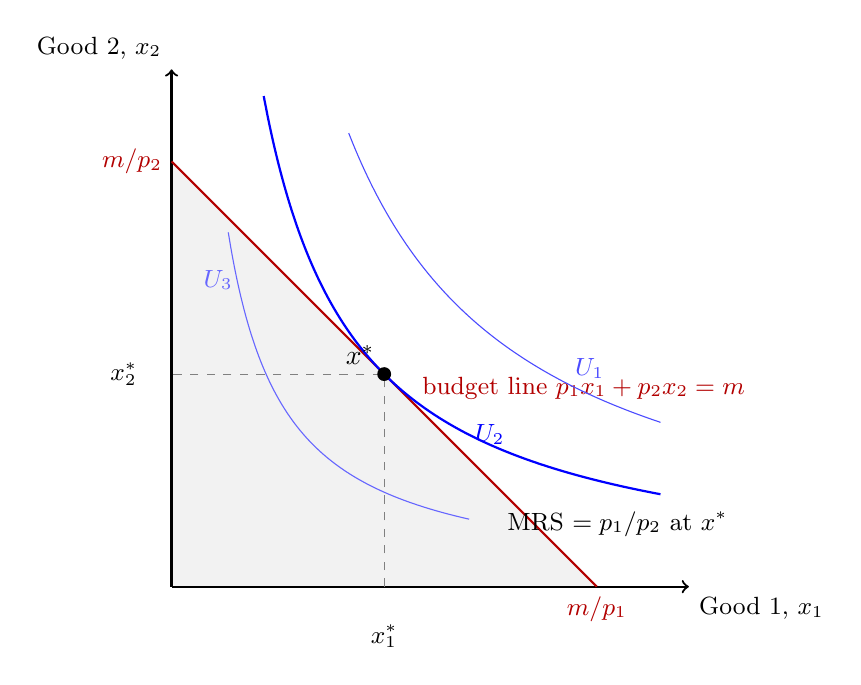
\begin{tikzpicture}[x=0.9cm, y=0.9cm]
  % convex budget (feasible) set
  \fill[gray!10] (0,0) -- (0,6) -- (6,0) -- cycle;
  % axes
  \draw[thick, ->] (0,0) -- (7.3,0) node[below right, font=\small] {Good 1, $x_1$};
  \draw[thick, ->] (0,0) -- (0,7.3) node[above left, font=\small] {Good 2, $x_2$};
  % budget line
  \draw[thick, red!70!black] (0,6) -- (6,0);
  \node[red!70!black, font=\small, left] at (0,6) {$m/p_2$};
  \node[red!70!black, font=\small, below] at (6,0) {$m/p_1$};
  \node[red!70!black, font=\small, below right] at (3.4,3.1) {budget line $p_1 x_1 + p_2 x_2 = m$};
  % indifference curves (convex to origin)
  \draw[blue!60] plot[domain=0.8:4.2, samples=80, smooth] (\x, {4/\x});
  \draw[blue, thick] plot[domain=1.3:6.9, samples=80, smooth] (\x, {9/\x});
  \draw[blue!70] plot[domain=2.5:6.9, samples=80, smooth] (\x, {16/\x});
  % optimum
  \draw[dashed, thin, gray] (3,0) -- (3,3) -- (0,3);
  \fill (3,3) circle (2.5pt) node[above left] {$x^{*}$};
  \node[font=\small, below] at (3,-0.4) {$x_1^{*}$};
  \node[font=\small, left] at (-0.35,3) {$x_2^{*}$};
  % labels
  \node[blue!60, font=\small, above left] at (1,4.05) {$U_3$};
  \node[blue, font=\small, right] at (4.15,2.15) {$U_2$};
  \node[blue!70, font=\small, above] at (5.9,2.8) {$U_1$};
  \node[font=\small, below right] at (4.6,1.2) {MRS $= p_1/p_2$ at $x^{*}$};
\end{tikzpicture}
\end{document}
